\documentclass[10pt,oneside,a4paper]{article}
\usepackage[IL2]{fontenc} % lepšia sadzba písmena Ľ než v T1
\usepackage[utf8]{inputenc}
\usepackage{graphicx}
\usepackage{url} % príkaz \url na formátovanie URL
\usepackage{hyperref} % odkazy v texte budú aktívne (pri niektorých triedach dokumentov spôsobuje posun textu)

\usepackage{cite}

\pagestyle{headings}
\title{Procedural Game Content Generation Using the Wave Function Collapse Algorithm\thanks{Semester project in the subject Methods of engineering work, year 2022/23, management: Name Surname}}
\author{Martin Dinja\\[2pt]
	{\small Slovak University of Technology in Bratislava}\\
	{\small Faculty of Informatics and Information Technologies}\\
	{\small \texttt{xdinja@stuba.sk}}
}

\date{\small 30.\ september 2022}

\begin{document}

\maketitle

% \tableofcontents

\begin{abstract}
    \begin{center}
        This thesis deals with the problem of generating game content using the Wave Function Collapse algorithm. The algorithm is described in detail and its application to the generation of game content is demonstrated. The thesis also contains a comparison of the algorithm with other methods of generating game content.
    \end{center}
\end{abstract}

\section{Introduction}\label{sec:introduction}

% An Introduction to the application of the wave function collapse algorithm for procedural generation of game content.
Procedural content generation (PCG) is a general term for a system that follows some patterns and generates an output based on those patterns.
Its main use case is generating assets or content that would be too time-consuming to create manually.
PCG is mainly connotatively tied to game content generation, but its use cases can be more creative.
Most PCG systems use game-specific assets with game-specific rules and algorithms to generate their content.
A more general application fit for a wide range of games is the Wave Function Collapse algorithm developed by Maxim Gumin~\cite{WFC}.
Wave Function Collapse is a greedy PCG algorithm based on the concept of collapsing a wave function, which is a mathematical representation of a quantum state.
This method can generate a large, high-quality, consistent output from a small set of input patterns.
It can be used in various applications, although its most commonly used for generating 2D tilemaps for games.
It can also generate 3D models, music, poetry, and more.
WFC's output can only be as good as its input, so it's essential to have a good set of input patterns and rules. 
My goal in this thesis is to create a simple, configurable application that will use the WFC algorithm to generate tilemaps for games, given a user-defined set of input patterns and rules.

\section{Theory}\label{sec:theory}
% Theoretical background of the wave function collapse algorithm.
As mentioned in the introduction [\ref*{sec:introduction}], the Wave Function Collapse algorithm is a greedy PCG algorithm based on the concept of collapsing a wave function, which is a mathematical representation of a quantum state.
A function starts in a superposition of values and collapses when that function is measured.
The result of the measurement is the value of the function at that point.
We can apply that concept for the generation of 2D tilemaps.
First, we need to define a set of input patterns and their rules regarding each other.
Then the algorithm will assign each tile a superposition of all possible patterns.
After prepending the superpositions, the algorithm will assign one random pattern to a tile with the least superpositions, also known as the least entropy, effectively collapsing its wave function, which is also why it is called a collapse algorithm.
Then we reevaluate all the affected tiles and their possible patterns and remove the ones that don't fit the rules.
Then we repeat the process until there is no more entropy in the tilemap.
This all is explained in more detail in Boris's article~\cite{WFCE}.

\section{Extensions}\label{sec:extensions}
Other then the most basic implementation of the algorithm, we also have extensions to the algorithm that allow us to generate more complex content.
For example, we can have a different shaped grid, different constraints and ways of looking at those constraints.

\subsection{The Overlap Model}
The most notable extension is the Overlap Model, which is mainly used to generate 2D textures.
Here we input a image which will act as our input pattern.
And, when it comes to rules, instead of concerning ourselves with the adjacency of tiles, we compare a 3$\times$3 group of tiles of our output to a 3$\times$3 group of our input pattern.
This produce a variation of the input pattern.
However, no matter how intuitive it is, it also is harder to implement, slower, and less flexible than the tiling model.
This extension is also not used in this implementation.

\subsection{Semi-Automatic Rule System}\label{sec:semi-automatic_rule_system}
Rather than detailing every relation to every possible rotation of every tile. We use an array of four numbers representing a connection type for each side of the tile. \texttt{[top, right, bottom, left]}.
Only the same connection types are allowed to connect to each other.
The system than automatically generates all the possible rotations of the tile and their connections.
We can also define which tile can connect to which other tile. Making sure that for even if the connection types match, we can still prevent the tiles from connecting to each other if needed.

\begin{figure}[ht]
    \centering
    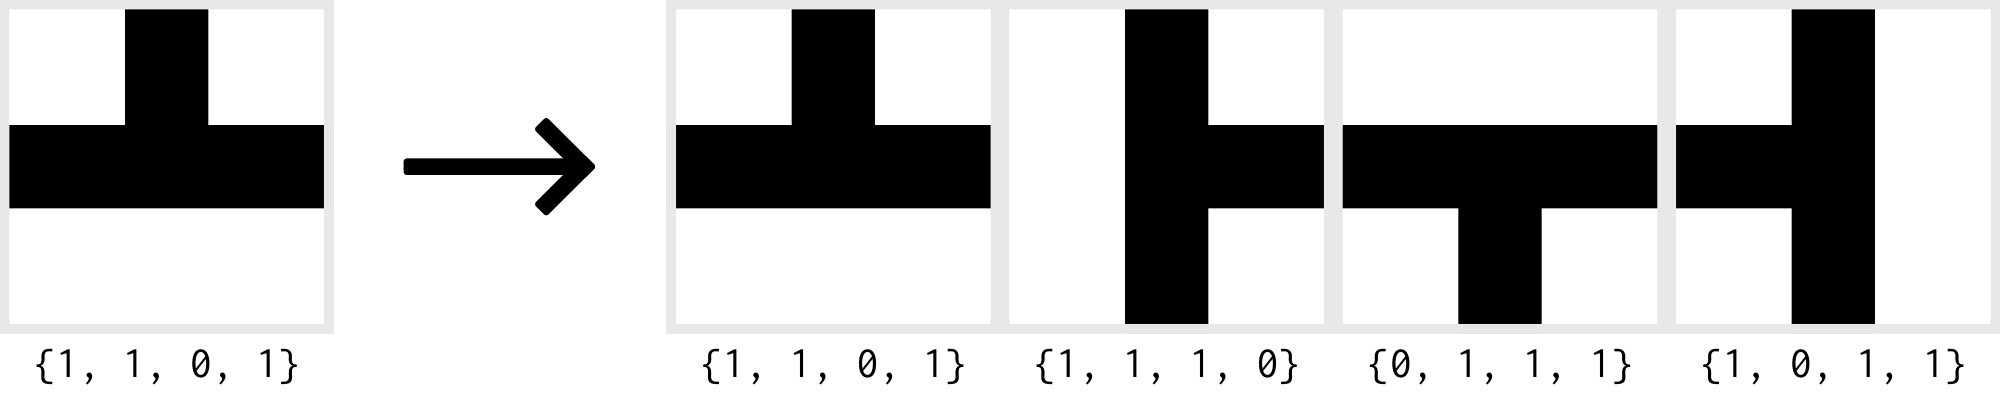
\includegraphics[width=0.8\textwidth]{figures/tile_rotation_example.png}
    \caption{Tile Rotation}\label{fig:tile_rotation_example}
\end{figure}


\section{Algorithm Implementation}\label{sec:implementation}
The model we are using is the tiling model, because it can be manually configured with more complex constraints making it more suitable for game content generation.
With it we also use a custom semi-automatic rule system extension, which was mentioned in the previous section [\ref*{sec:semi-automatic_rule_system}].

The central part of the project is the algorithm itself.
It uses the helper, interface, and infrastructure functions to work with the tile grid.
It starts by inferring all the rules with the semi-automatic rule system[\ref*{sec:semi-automatic_rule_system}].
Then it initialize the tile grid and fill each tile's state array with all possible states.
And the the main loop of the algorithm starts.
In the loop, we get the tile with the least entropy, collapse it, and reevaluate all the affected cells.
Evaluating the cells is done by updating the states of each neighbor of the collapsed cell, then reevaluating the states of their neighbors, and so on, until we reach a point where cell states don't change any more.
Finally, we check if all of the cells are collapsed, and if they are, the algorithm halts.
Otherwise, we repeat the loop.

\begin{figure}[ht]
    \centering
    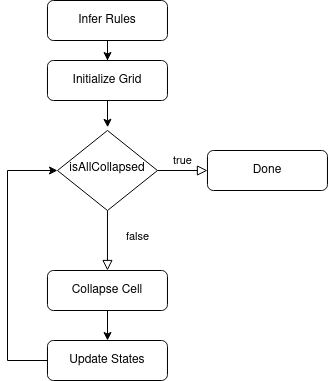
\includegraphics[width=0.6\textwidth]{figures/model_loop_diagram.png}
    \caption{Model Loop Diagram}\label{fig:model_loop_diagram}
\end{figure}


\section{Results}\label{sec:results}
% subsections: examples, performance, conclusions.
With the algorithm implemented, we can now generate tilemaps.
Starting off with a simple example (Figure~\ref{fig:example1}).
\begin{figure}[ht]
    \centering
    
\includegraphics[width=0.5\textwidth]{figures/road_tiles.png}
    \caption{Road Tiles}\label{fig:example1}
\end{figure}

Defining the rules for these tiles, we can generate a 10 by 10 tilemap with the following result (Figure~\ref{fig:example1map}):
The generation shouldn't take more than a second.

\begin{figure}[ht]
    \centering
    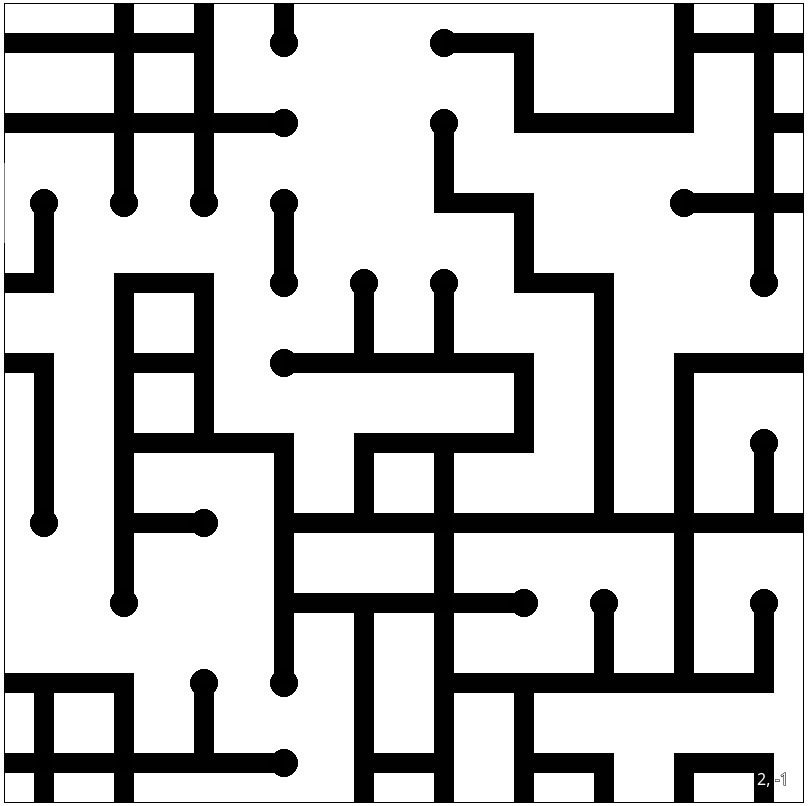
\includegraphics[width=0.5\textwidth]{figures/roads_output.png}
    \caption{Road Output}\label{fig:example1map}
\end{figure}

Altho the algorithms is very simple, it tends to break when the rule-set is more complex, and when the grid size is bigger.
This is due to the fact that the algorithm is greedy and it tends to collapse the most common patterns first, which can lead to a lot of dead-ends.

Optimizations can be made to the algorithm, and the rule system can be expanded to support more complex rules.
There is a lot of room for improvement, but for now, it is a good start.

\section{Modifications}\label{sec:modifications}
% Modifications to the algorithm.
The algorithm is very simple and straightforward, but it can be modified to fit different needs.
For a more controlled distribution of tile types we can assign a weight value to each type.
The weight value will be used to determine the likelihood of a tile being collapsed into a certain pattern.

We can also expand WFC with generic search, giving it the ability to generate levels targeting specific play experiences.
This is the topic of a paper released by Raphael Bailly and Guillaume Levieux\cite{BL22}.

There is also a way to augment the algorithm with the Growing Grid neural network for procedural map generation~\cite{NMBP20}

We can take control to another level and introduce more constraints to the algorithm making the output seem more Human-Designed.
As detailed in the paper by Darui Cheng, Honglei Han, and Guangzheng Fei\cite{CHF20}.

And Of course there are many more ways to modify the algorithm for different purposes.

\section{Comparison with other methods}\label{sec:comparison}
% subsections: other methods, pros and cons.

There are many different procedural content generation (PCG) algorithms that are similar to the Wave Function Collapse (WFC) algorithm, each with its own strengths and limitations.
Some of them are more suited for more specific tasks, while others are more general.
Some are faster, while others are slower. Some are more complex, while others are simpler.
Comparing them is a difficult task, since they have wildly different approaches and goals.
But we can still compare WFC to some of the more related methods.
Some examples of these algorithms include:
\begin{itemize}
    \item Model synthesis, which uses a set of rules and constraints to generate 3D models
    \item Perlin noise, which uses random noise functions to generate smooth, natural patterns or textures that can be used as input for other PCG algorithms
    \item Markov chain algorithms, which use statistical models to generate sequences of symbols or events based on the probabilities of their occurrences in the input data
    \item Genetic algorithms, which use principles of natural evolution to generate new solutions or configurations by combining and mutating existing ones
    \item L-systems, which use a set of rules and symbols to generate complex structures or patterns based on repeated applications of the rules
\end{itemize}
Each of these algorithms has its own unique characteristics and capabilities, and can be used in a variety of applications, including game content generation.

Let's talk a bit about Model Synthesis, which is a constraint-based algorithm mainly used for generating 3D models.
Paul Merrell, the creator of model synthesis has compared the two algorithms in his paper\cite{Mer21}.
\begin{quote}
    \textit{Model synthesis and WFC use nearly the same algorithm and produce similar results. WFC picks cells in a different
order and does not modify in blocks. This causes the algorithm to fail more on some large models.}
\end{quote}

When it comes to comparing WFC and Perlin noise, the main difference is that WFC uses a random process known as the ``collapse'' of a wave function to determine which input patterns are selected and combined to create the output, while Perlin noise uses a random noise function to generate smooth, natural-looking patterns or textures.

There are a lot of similarity with the other algorithms, but the main differences are the types of mathematical models used to generate the output.
Even tho each algorithm can be configured to generate different types of content, they are all very different in how they work.
WFC is commonly used for generating 2D tilemaps for games, but can also be applied to other types of content.
Markov chain algorithms can be used to generate a wide range of outputs, including text, music, and images.
Genetic algorithms are commonly used to solve optimization problems, and can be applied to a wide range of domains, including game content generation.
And L-systems are commonly used to model the growth of plants and other natural systems, and can be applied to generate 2D and 3D graphics, as well as other types of content.

\section{Conclusion}\label{sec:conclusion}
In this thesis, we had a brief introduction to PCG algorithms.
We then went over the Wave Function Collapse algorithm, and its implementation.
We explained in detail how the algorithm works, a way to implemented it, and how it can be modified.
We also showed some examples of the algorithm in action, and compared it to some other PCG algorithms.
WFC is a very simple algorithm, but it's very powerful and can be used to generate a wide variety of content.
It also has a very simple implementation, and can be easily modified to fit different needs.
It's a great algorithm to start with when learning about PCG\@.

\bibliography{lit}
\bibliographystyle{alpha}

\end{document}
